\UseRawInputEncoding
\documentclass[12pt]{report}
\usepackage[utf8]{inputenc}
\usepackage[french]{babel}
 \usepackage{multirow} 
\usepackage{graphicx}
\usepackage{array}
 \usepackage{enumitem}
 \usepackage{inputenc}
\usepackage{pifont}
\usepackage{float} 

\usepackage{shorttoc}
\usepackage{amsmath}
\usepackage{csquotes}
\usepackage{tocloft}
\usepackage{endnotes}
\let\footnote=\endnote
%\usepackage{titlesec}
\usepackage[pagestyles]{titlesec}
\usepackage[Lenny]{fncychap}
\renewcommand{\thesection}{\arabic{chapter}.\arabic{section}.}
\renewcommand{\thesubsection}{\arabic{chapter}.\arabic{section}.\arabic{subsection}}
\renewcommand{\thesubsubsection}{\arabic{chapter}.\arabic{section}.\arabic{subsection}.\arabic{subsubsection}}
%\renewcommand{\thesubsubsection}{\thesubsection.\arabic{subsubsection}}
\usepackage[ margin=1in]{geometry}
%\usepackage [style=ieee]{biblatex}
\usepackage[
  style=numeric-comp,
  %style=ieee,
  datamodel=software, % extend the datamodel with entries for software
  abbreviate=false,
  natbib=true,
	%sortlocale=auto,
  %sorting=ynt,
  sorting=none,
  %backend=biber,
  backend=bibtex,
  bibencoding=utf8,
  %giveninits=true,
  url=true,
  doi=true,
  defernumbers,
  maxcitenames=3,
  defernumbers=false,
  maxbibnames=100]{biblatex}
%\addbibresource{bibitem.bib}
\renewcommand{\baselinestretch}{1.5}
\usepackage[T1]{fontenc} 



% Set depth for numbering levels
\setcounter{secnumdepth}{2}

\usepackage{fancyhdr}
\pagestyle{fancy}
%\fancyhead[L]{\leftmark}
%\fancyhead[R]{machin}
\fancyhead[L]{Université Joseph KI-ZERBO (UJKZ)}
\fancyhead[R]{Année académique 2024-2025}
\renewcommand{\footrulewidth}{0.4pt}
\fancyfoot[L]{OUEDRAOGO D David Lucas 1er Jumeau}
\fancyfoot[R]{Mémoire de Master}
\bibliography{bibitem} 
\usepackage{nomencl}
\usepackage{caption}
\usepackage{xcolor}
\usepackage{colortbl}

\usepackage{tikz}
\usetikzlibrary{positioning,shapes.geometric,arrows.meta,calc}
%\usetikzlibrary{shapes,arrows,positioning,calc}

\usepackage{geometry}
\usepackage{longtable}
%\usepackage{hyperref}
\geometry{a4paper, total={170mm,257mm}, left=20mm, top=20mm}
\usepackage{booktabs}
\setlength{\parindent}{0pt}


\newcolumntype{P}[1]{>{\centering\arraybackslash}p{#1}}



%\usepackage{hyperref}
%\usepackage{minitoc}
%\usepackage{uarial}
%\usepackage{lmodern}
%\usepackage{cmbright}

%\usepackage{fontspec}
%\setmainfont{texgyrebonum-regular.otf}
%\setsansfont{lmsans10-regular.otf}[Scale=MatchLowercase]
%\setmonofont{Inconsolatazi4-Regular.otf}[Scale=MatchLowercase]

%\usepackage[T1]{fontenc}
%\usepackage{uarial}
%\renewcommand{\familydefault}{\rmdefault}

\makenomenclature

\definecolor{myColor}{rgb}{0,0.1,0.55} 
%\definecolor{myColor}{rgb}{0.75,0,0.59}
%\definecolor{myColor}{rgb}{0,0.4,0.5} 
\usepackage[colorlinks=true,linkcolor=myColor,citecolor=myColor,urlcolor=myColor]{hyperref}

\colorlet{defaultcolor}{black!75!myColor} % Define your default color here
%\definecolor{defaultcolor}{rgb}{0,0.32,0.5}
\color{defaultcolor} % Set default color for the whole document

\newcommand{\hlinecolor}{\arrayrulecolor{myColor}\hline\arrayrulecolor{black}}


%\titleformat{\chapter}[display]
  %{\normalfont\rmfamily\huge\bfseries\scshape\color{myColor}}
  %{\chaptertitlename\ \thechapter}{20pt}{\Large}
	
\renewcommand{\thechapter}{\Roman{chapter}}
\titleformat{\chapter}[display]
{\normalfont\Large\filcenter\rmfamily \bfseries \scshape \color{myColor}}
{\titlerule[1pt]%
\vspace{1pt}%
\titlerule
\vspace{1pc}%
%\LARGE\MakeUppercase{\chaptertitlename} \thechapter}
\Large \chaptertitlename\ \thechapter}
{1pc}
{\titlerule
\vspace{1pc}%
\Large}

\titleformat{\section}
  {\normalfont\rmfamily\Large\bfseries \color{myColor}}
  {\thesection}{1em}{}

\titleformat{\subsection}
  {\normalfont\rmfamily\large\bfseries \color{myColor}}
  {\thesubsection}{1em}{}

\titleformat{\subsubsection}
  {\normalfont\rmfamily\large\bfseries \color{myColor}}
  {\thesubsubsection}{1em}{}
	
\titleformat{\figure}
  {\normalfont\rmfamily\large\bfseries \color{myColor}}
	{\figurename}{1em}{}


% Set the color for the entire caption
\captionsetup[figure]{font={color=myColor},justification=centering}
\captionsetup[table]{font={color=myColor},justification=centering}
\captionsetup[equation]{font={color=myColor}}
	
	%\titleformat{<command>}[<shape>]{<format>}{<label>}{<sep>}{<before-code>}[<after-code>]

 %Utilisation de \linespread pour augmenter l'espacement des lignes
\linespread{1.25}



\renewcommand{\familydefault}{\sfdefault}
%\renewcommand{\familydefault}{\rmdefault}


\title{Mémoire de Master 2 : [Insert Subject]}
\author{KABORE W. Cédric B.}
\date{Septembre 2025}
\graphicspath{{ps/}{fig/}}

%--------------------------------------------

\usepackage{listings}
\usepackage{color}

\definecolor{codegreen}{rgb}{0,0.6,0}
\definecolor{codegray}{rgb}{0.5,0.5,0.5}
\definecolor{codepurple}{rgb}{0.58,0,0.82}
%\definecolor{backcolour}{rgb}{0.95,0.95,0.92}
\definecolor{backcolour}{rgb}{0.97,0.97,0.97}

\lstdefinestyle{mystyle}{
    backgroundcolor=\color{backcolour},   
    commentstyle=\color{codegreen},
    keywordstyle=\color{magenta},
    numberstyle=\tiny\color{codegray},
    stringstyle=\color{codepurple},
    %basicstyle=\footnotesize,
		%basicstyle=\ttfamily\footnotesize,
		basicstyle=\ttfamily,
    breakatwhitespace=false,         
    breaklines=true,                 
    captionpos=b,                    
    keepspaces=false,                 
    numbers=left,                    
    numbersep=5pt,                  
    showspaces=false,                
    showstringspaces=false,
    showtabs=false,                  
    tabsize=1
}
\lstset{style=mystyle}



%--------------------------------------------

\begin{document}

%=========================== [Page de garde]=======================
\begin{titlepage}

\vspace {10.0cm}

\begin{center}
%{\bf Ministère de l’Enseignement Supérieur, de la Recherche Scientifique et de l’Innovation} \vspace{0.1cm}\\
%
%{\bf UNIVERSITÉ JOSEPH KI-ZERBO} \vspace{0.1cm}\\
%
%{\bf {\large Unité de Formation et de Recherche en Sciences Exactes et Appliquées (UFR-SEA) \vspace{0.1cm} }}\\
%
%{\bf Département d’Informatique }\vspace{0.1cm} \\
%
%{ \textbf{Laboratoire de Mathématiques et d’Informatique (LAMI)}}\\ \vspace{0.2cm}

%------------------------------------------------------------------------- 06
%------------------------------------------------------------------------  04
\Large{\textbf{UNIVERSITÉ JOSEPH KI-ZERBO (UJKZ)}} \\
\rule{.50\linewidth}{0.5pt}
\\
\vspace{0.25cm}
\large{\textsc{\textbf{Unité de Formation et de Recherche (UFR) \\en Sciences Exactes et Appliquées (UFR-SEA)}}}
\rule{.50\linewidth}{0.5pt}
\\
\vspace{0.25cm}
\textbf{Laboratoire de Mathématiques et d’Informatique (LAMI)}


%\begin{figure}[htbp]
%\centering
 %\hbox{
     %\includegraphics[width=125px]{uo}
     %\hspace*{2.0cm}
     %\includegraphics[width=175px]{sea}
     %%\hspace*{0.5cm}
     %%\includegraphics[width=150px]{lami.jpeg}
  %}
%\end{figure}

\begin{figure}[htbp]
\centering

\includegraphics[width=0.99\textwidth]{image/lami.jpeg}
\end{figure}

%\Huge{\textbf{Mémoire de Master}} \\   \vspace{0.3cm}
%\Huge{\textbf{MÉMOIRE DE MASTER}} \\   \vspace{0.3cm}
\large{\textsc{\textbf{Mémoire de Master}}}

%\large{{\textbf{Domaine: }Sciences et technologies }}\\ \vspace{0.1cm}
%\large{{\textbf{Mention:} Informatique  }}\\ 
%\large{ \textbf{Option :}  Systèmes, Réseaux et Télécommunication (SRT)}\\

\begin{center} 
\begin{tabular}{p{0.95\textwidth}} 
\centering \large{ \textbf{Domaine:}}   \large{ Sciences et Technologies } \\
\centering \large{ \textbf{Mention:}}   \large{ Informatique }  \\
\centering \large{ \textbf{Option :}}   \large{ Sécurité Informatique et Cybersécurité (SIC) }
\end{tabular}
\end{center}



\large{ {Année académique 2024-2025}\\ }
%\Large{\textbf{Thème}}\\ 
\textcolor{blue}{\noindent\rule{\textwidth}{0.25mm}}
\large{\textbf{\textcolor{myColor}{DÉTECTION DES MALWARES VIA UNE
BLOCKCHAIN COLLABORATIVE }}}
\textcolor{blue}{\noindent\rule{\textwidth}{0.25mm}}
\end{center}
\vspace{0.3cm}



%-------------------------------------------------------------------------- 07
%\begin{tabular}{ p{6cm}  p{6cm}  p{6cm}}
%\begin{tabular}{*{20}{l}}
%\begin{tabular}{p{0.333\textwidth} p{0.333\textwidth} p{0.333\textwidth}} 

\begin{tabular}{>{\centering\arraybackslash}p{\textwidth}} 

% Bloc Étudiant
\textbf{Soutenu par :} \\
M. OUEDRAOGO Delwende David Lucas 1er Jumeau  \\ [4ex] 

% Bloc Direction
\textbf{Sous la direction de :} \\
Dr Didier BASSOLE \\

\end{tabular}

\begin{center} 
\textbf{Soutenu le .... 2024 devant le jury composé de :}
\end{center}
\vspace*{0.3cm}

\begin{tabular}{p{0.16\textwidth} p{0.28\textwidth} p{0.7\textwidth}} 

\textbf{Président :} & Dr .... & Maître de Conférences, Université Joseph KI ZERBO\\
\textbf{Encadrant :} & Dr Zakaria SAWADOGO & Maître Assistant, Université Jeseph KI ZERBO\\
\textbf{Examinateur :} & Dr ..... & Maître Assistant, Université Jeseph KI ZERBO\\
\textbf{Rapporteur :} & Dr .... & Assistant, Université Jeseph KI ZERBO\\
\end{tabular}
\\

\end{titlepage}

%%=========================== [Déclaration sur l’honneur]=======================
% \vspace*{3cm}
% \section*{Déclaration sur l'honneur}
% \vspace*{1cm}

% Je soussigné \textcolor{myColor}{KABORE W Cédric B} certifie par la présente que le mémoire portant sur la \textcolor{myColor}{Approche de gestion sécurisée de certificats numériques IoT, basée sur la thecnologie blockchain} ainsi que les travaux qui y sont présentés sont le fruit de mon propre travail. J'affirme ce qui suit :
% \begin{itemize}
% 	\item  ce travail a été réalisé en totalité ou en grande partie dans le cadre de mes études en Master à l'Université Joseph KI ZERBO ;
% 	\item  tout élément préalablement soumis en vue de l'obtention d'un diplôme ou de toute autre qualification au sein de cette université est clairement mentionné ;
% 	\item  Lorsque j'ai utilisé des travaux publiés par d'autres auteurs, j'ai rigoureusement indiqué leurs sources ;
% 	\item  les références sont systématiquement fournies lors de toute citation provenant du travail d'autrui. À l'exception de ces citations, l'intégralité de ce travail est le résultat de mes propres initiatives ;
% 	\item  j'ai pleinement identifié toutes les sources principales de soutien. En cas de collaboration avec d'autres personnes, j'ai explicitement exposé les contributions respectives en détaillant les réalisations individuelles.
% \end{itemize}

% \vspace*{1cm}
% \textcolor{myColor}{\noindent\rule{0.75\textwidth}{0.25mm}}

% \begin{description}
% 	\item [Date :]
% 	\item []
% 	\item [Signé :]
% \end{description}
%%=========================== [Dédicace]=======================
%\chapter*{Dédicace}
\newpage
\section*{Dédicace}
\pagenumbering{Roman}
\setcounter{page}{2}
\addcontentsline{toc}{chapter}{Dédicace}

\textsl{\colorbox[rgb]{1,1,0}{TO BE UPDATED ...}}

\thispagestyle{fancy}
\vspace{2cm}

\begin{center}
À ma famille,\\
à mes enseignants,\\
et à tous ceux qui ont contribué à la réalisation de ce travail.
\end{center}

\newpage
\newgeometry{left=2.25cm,top=2.2cm,bottom=2.2cm}

%%=========================== [Remerciements]=======================
%\chapter*{Remerciements}
\section*{Remerciements}
\addcontentsline{toc}{chapter}{Remerciements}

Je tiens à exprimer ma profonde gratitude à :
\begin{itemize}
    \item mon encadrant pour ses conseils et sa disponibilité ;
    \item mon superviseur pour son accompagnement scientifique ;
    \item le corps enseignant du Département d’Informatique ;
    \item l’UFR-SEA pour le cadre académique offert ;
    \item mes camarades de laboratoire pour l’entraide ;
    \item ma famille pour son soutien moral.
\end{itemize}
\textsl{\colorbox[rgb]{1,1,0}{TO BE UPDATED ...}}

\thispagestyle{fancy}

%%=========================== [Abréviations]=======================
\newpage
\newgeometry{left=2.25cm,top=2.2cm,bottom=2.2cm}
%\renewcommand{\nomname}{Liste des abréviations}
%Liste des abréviations}
%\renewcommand{\nomname}{\addcontentsline{toc}{chapter}{Liste des abréviations}Liste des abréviations}

%\nomenclature{ADC}{	convertisseur analogique numérique} 
%\printnomenclature
%\thispagestyle{fancy}
%\restoregeometry

\section*{Liste des abréviations}
\addcontentsline{toc}{chapter}{Liste des abréviations} \setcounter{page}{4}

\begin{tabular}{p{0.135\textwidth} p{0.750\textwidth}}  \hlinecolor

\raggedright \textcolor{myColor}{AI: } &  Artificial Intelligence (Intelligence Artificielle)    \\
\raggedright \textcolor{myColor}{CNN: } &  Convolutional Neural Network (Réseau Neuronal Convolutif)   \\
\raggedright \textcolor{myColor}{DNN: } &  Deep Neural Network (Réseau Neuronal Profond)   \\
\raggedright \textcolor{myColor}{DL: } &  Deep Learning (Apprentissage Profond)  \\
\raggedright \textcolor{myColor}{DRL: } & Deep Reinforcement Learning (Apprentissage par Renforcement Profond)  \\
\raggedright \textcolor{myColor}{FPS: } & Frames Per Second (Images par Seconde) \\
\raggedright \textcolor{myColor}{GNSS: } & Global Navigation Satellite System (Système Mondial de Navigation par Satellite) \\
\raggedright \textcolor{myColor}{GPU: } & Graphics Processing Unit (Processeur Graphique) \\
\raggedright \textcolor{myColor}{IoU: } & Intersection over Union (Méthode d’Évaluation des Détections) \\
\raggedright \textcolor{myColor}{IoT: } & Internet of Things (Internet des Objets) \\
\raggedright \textcolor{myColor}{LIDAR: } & Light Detection And Ranging (Télédétection par Laser) \\
\raggedright \textcolor{myColor}{mAP: } & Mean Average Precision (Précision Moyenne Moyenne) \\
\raggedright \textcolor{myColor}{ML: } & Machine Learning (Apprentissage Automatique) \\
\raggedright \textcolor{myColor}{NLP: } & Natural Language Processing (Traitement du Langage Naturel) \\
%\raggedright \textcolor{myColor}{PRACH: } &  Physical Random Access Channel (Canal d'Accès Aléatoire Physique) \\
\raggedright \textcolor{myColor}{RF: } & Radio Frequency (Fréquence Radio) \\
\raggedright \textcolor{myColor}{RNN: } & Recurrent Neural Network (Réseau de Neurones Récurrent) \\
\raggedright \textcolor{myColor}{SNR: } & Signal-to-Noise Ratio (Rapport Signal-Bruit) \\
\raggedright \textcolor{myColor}{SORT: } & Simple Online and Realtime Tracker (Suivi en Temps Réel et en Ligne) \\
\raggedright \textcolor{myColor}{SSD: } & Single Shot MultiBox Detector (Détecteur Multi-Boîtes à Prise Unique) \\
\raggedright \textcolor{myColor}{TPU: } & Tensor Processing Unit (Processeur de Traitement Tensoriel) \\
\raggedright \textcolor{myColor}{UAV: } & Unmanned Aerial Vehicle (Véhicule Aérien Sans Pilote - Drone) \\
\raggedright \textcolor{myColor}{UAS: } & Unmanned Aerial System (Système Aérien Sans Pilote) \\
%\raggedright \textcolor{myColor}{URLLC: } & Ultra-Reliable and Low Latency Communications (Communications Ultra-Fiables et à Faible Latence) \\
\raggedright \textcolor{myColor}{VLOS: } & Visual Line of Sight (Ligne de Vue Visuelle) \\
\raggedright \textcolor{myColor}{YOLO: } & You Only Look Once (Modèle de Détection d'Objets en Une Seule Passe) \\

\hlinecolor
\end{tabular}



%%===================================================================


%\input{dedicace} 
%\input{remercie}
%\newpage
%\input{abreviation}
%\addcontentsline{toc}{chapter}{Liste des abréviations} \setcounter{page}{4}
%\input{resume}
%%=========================== [Résume]===============================
\newpage
%\chapter*{Résumé}
\section*{Résumé}
%\renewcommand{\abstractname}{\chapter*{Résumé}}
\addcontentsline{toc}{chapter}{Résumé}
\textsl{\colorbox[rgb]{1,1,0}{TO BE UPDATED ...}}
\\
\textbf{Mots clés :} XXX.
\thispagestyle{plain}
\setcounter{page}{5}
%\end{abstract}
%\selectlanguage{french}
\thispagestyle{fancy}
\newpage
%%=========================== [Abstract]===============================
 %\selectlanguage{english} 
 %\chapter*{Abstract}
 \section*{Abstract}
%\renewcommand{\abstractname}{\chapter*{Abstract}}
\addcontentsline{toc}{chapter}{Abstract}\textsl{\colorbox[rgb]{1,1,0}{TO BE UPDATED ...}}
\\
\textbf{Keywords :}  XXX.
%\thispagestyle{plain}
%\setcounter{page}{5}
%\end{abstract}
%\selectlanguage{french}
\thispagestyle{fancy}
%%===================================================================



%\input{abstract}
\setcounter{page}{6}
\newpage
\addcontentsline{toc}{chapter}{Sommaire}
\setcounter{page}{7}
\shorttableofcontents{Sommaire}{1}
\thispagestyle{fancy}

\newpage 
\listoffigures
\thispagestyle{fancy}
\addcontentsline{toc}{chapter}{Table des figures}
\newpage 
\listoftables
\thispagestyle{fancy}
\addcontentsline{toc}{chapter}{Liste des tableaux}



 
\newpage
\addcontentsline{toc}{chapter}{Introduction Générale}
\chapter*{Introduction Générale}
\thispagestyle{fancy}
\pagenumbering{arabic}
\setcounter{page}{1}
\paragraph{}Contexte 
\paragraph{}Problématique 
\paragraph{}OG : Afin d’apporter une réponse concrète à la problématique posée, notre étude se fixe pour objectif général .......:
\begin{itemize} 
    \item•	OS1 : Faire ......;
    \item•	OS2 : Proposer .....;
    \item•	OS3 : Évaluer la performance ....
\end{itemize}
\paragraph{}La suite de ce travail est structurée de manière progressive et cohérente.
 \begin{itemize} 
     \item Le premier chapitre est consacré à une revue exhaustive de la littérature, au cours de laquelle sont présentés les concepts fondamentaux du domaine étudié ainsi qu’une analyse critique des travaux existants. 
    \item• Le deuxième chapitre présente la démarche méthodologique adoptée et décrit l’approche proposée, conçue pour répondre de manière pertinente aux insuffisances identifiées dans l’état de l’art. 
    \item•	Le troisième chapitre est dédié à l’implémentation de la solution retenue, , à la conduite des expérimentations ainsi qu’à l’analyse approfondie et à l’interprétation des résultats obtenus. Enfin ce travail se conclut par une discussion générale et par la présentation des perspectives de recherche susceptibles d’orienter les travaux futurs.
 \newpage



%=======================
\chapter{Revue de la littérature}
\section{Concepts fondamentaux}

\subsection{Les Fondamentaux }

L'Internet des Objets (IoT) peut être défini comme un réseau .......

\subsubsection{Architecture Multi-couches et Surface d'Attaque}
L'architecture de l'IoT est conventionnellement structurée en plusieurs couches interdépendantes.....

\begin{itemize}
    \item \textbf{Couche de Perception :} Composée de capteurs et d'actionneurs, elle assure la capture de données physiques de son environnement ou exécute des actions en réponse à des instructions. Comme le soulignent Neshenko et al. \cite{neshenko2019demystifying}, ces dispositifs sont souvent dépourvus de mécanismes de protection physique, les rendant vulnérables aux modifications de \textit{firmware} \cite{basnight2013firmware} et aux attaques par canaux auxiliaires (\textit{side-channel attacks}) \cite{biryukov2017side}.
    \item \textbf{Couche Réseau :} Elle garantit .... \cite{pielli2017game}.
    \item \textbf{Couche Transport :} Elle a pour rôle essentiel d'assurer ....
    \item \textbf{Couche de Traitement des Données :} Cette couche traite les informations au plus près des dispositifs (Edge Computing), soit localement, soit via des passerelles, afin de ne transmettre que les données essentielles vers les plateformes de \textit{cloud computing}.
    \item \textbf{Couche Application :} Elle assure l'exploitation des données pour fournir des services spécifiques à l'utilisateur final. Les vulnérabilités y sont souvent liées à des interfaces de gestion non sécurisées, facilitant l'exécution arbitraire de commandes.
\end{itemize}


\subsubsection{Menaces Émergentes et Botnets}
Le manque de sécurité native transforme les parcs IoT en cibles idéales pour la création de \textit{botnets}. Pan et al. \cite{pan2025torchlight} ont démontré que des millions d'appareils restent exposés à des exploits \textit{zero-day} facilitant leur enrôlement dans des réseaux de zombies. L'attaque record de 5,6 Tbps signalée par Cloudflare \cite{cloudflare_ddos_2025} illustre l'évolution de ces menaces : les variantes modernes du \textit{botnet} Mirai optimisent désormais l'utilisation de quelques milliers de nœuds compromis pour générer des volumes de trafic autrefois réservés à des réseaux de taille mondiale.


\subsubsection{Concepts Fondamentaux de la Cryptographie}
Afin d'expliciter cette définition, il convient de préciser plusieurs concepts fondamentaux :
\begin{itemize}
    \item \textbf{Le chiffrement asymétrique :} Mécanisme de cryptographie où chaque entité détient une paire de clés liées mathématiquement. La clé publique est diffusable librement, tandis que la clé privée doit demeurer confidentielle. Ce système repose sur la difficulté mathématique d'inférer la clé privée à partir de la clé publique (problème de la factorisation première).
    \item \textbf{Les fonctions de hachage :} Fonctions unidirectionnelles transformant une donnée d'entrée en une empreinte de taille fixe (\textit{digest}). Elles garantissent l'intégrité : il est aisé de calculer l'empreinte, mais techniquement impossible de retrouver la donnée d'origine à partir de celle-ci.
    \item \textbf{La signature numérique :} Elle constitue une preuve de l'intégrité du message et de l'authenticité de son origine. Le processus consiste à chiffrer l'empreinte du message avec la clé privée de l'expéditeur (voir Figure \ref{fig1}).
    \item \textbf{Le certificat numérique :} Document électronique attestant du lien entre une clé publique et une entité. Cette liaison est garantie par la signature numérique d'une Autorité de Certification (CA).
\end{itemize}

\begin{figure}[htb]
    \centering
    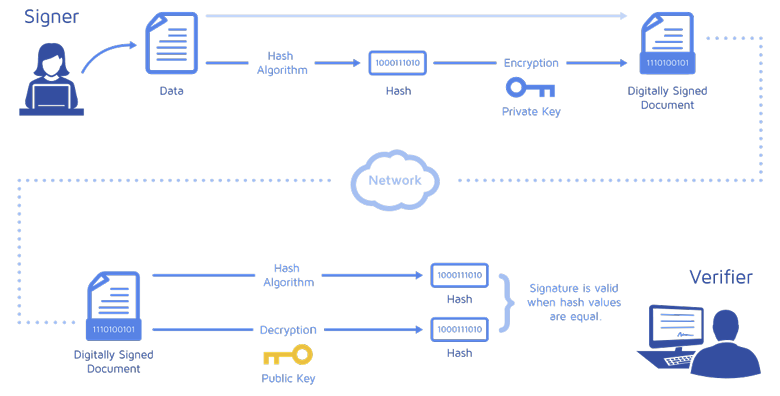
\includegraphics[width=\linewidth]{image/image.png}
    \caption{Processus de vérification de l'intégrité par signature numérique}
    \label{fig1}
\end{figure}


\subsection{La Technologie Blockchain : Vers une Décentralisation de la Confiance}

La blockchain s'impose comme une alternative disruptive aux modèles de confiance centralisés, offrant un cadre décentralisé pour la gestion des identités numériques.

\subsubsection{Définition et Principes Fondamentaux}
Inspirée par les travaux de Nakamoto \cite{nakamoto2008bitcoin}, la blockchain est un registre distribué (\textit{Distributed Ledger Technology} - DLT) stockant des informations de manière immuable, transparente et sécurisée. Son fonctionnement repose sur plusieurs piliers technologiques :
\begin{itemize}
    \item \textbf{Décentralisation :} Contrairement aux bases de données traditionnelles, le registre est répliqué sur un ensemble de nœuds indépendants, éliminant tout point de défaillance unique.
    \item \textbf{Immuabilité :} Chaque bloc de données est lié au précédent par une empreinte cryptographique (hachage). Toute modification rétroactive d'un bloc nécessiterait la reconfiguration de l'ensemble de la chaîne, rendant les données pratiquement inaltérables.
    \item \textbf{Mécanisme de Consensus :} Un protocole (tel que le \textit{Proof of Work} ou le \textit{Proof of Stake}) permet aux nœuds du réseau de s'accorder sur la validité des nouvelles données sans nécessiter d'entité centrale de contrôle.
\end{itemize}

\subsubsection{Automatisation par les Smart Contracts}
Le concept de \textit{Smart Contract}, ou contrat intelligent, introduit par Nick Szabo et popularisé par Ethereum, désigne des programmes autonomes qui s'exécutent automatiquement sur la blockchain lorsque des conditions prédéfinies sont remplies. Dans le contexte de la sécurité, ils permettent de traduire des politiques de confiance en code auto-exécutant, garantissant que les transactions (comme l'émission d'un certificat) respectent strictement les règles établies sans intervention humaine.



\section{Travaux connexes}

\paragraph{}La prolifération rapide des malwares et la complexité croissante ....

\begin{itemize}
 \item \textbf{Limites des antivirus traditionnels}
 \\
 \textbf{Aboaoja et al(2022)} [1], présente une analyse exhaustive des méthodes classiques ...... 
 \\
 Cette faiblesse a motivé les travaux de \textbf{Dimov et Savova (2024)} [2] ....
 \\
 \item \textbf{Méthodes dynamique et intelligentes de détection collaborative}
 \\
 Afin de dépasser les limites des approches statiques, plusieurs travaux récents se sont orientés vers des méthodes de détection dynamiques et intelligentes fondées sur l’analyse comportementale et l’intelligence artificielle. 
 \\
 Dans cette perspective, Mesut GÜVEN (2024) [3].....
 \\

\\
\begin{table*}[htbp]
\centering
\small
\renewcommand{\arraystretch}{1.4}
\begin{tabular}{|p{2cm}|p{2cm}|p{4.2cm}|p{5.3cm}|}
\hline
\textbf{Catégorie} & \textbf{Auteurs}  & \textbf{Forces} & \textbf{Faiblesses / Limites} \\ \hline

\multirow{2}{3cm}{Antivirus traditionnels} 
& Aboaoja et al. (2022) 
& Analyse comparative des signatures, heuristiques, sandbox et apprentissage automatique. 
& Forte dépendance aux signatures statiques ; inefficacité face aux malwares zero-day et polymorphes ; absence d’adaptativité. \\ \cline{2-4}

& Dimov \& Savova (2024) 
& Mise en évidence de l’efficacité de l’obfuscation multiple pour l’évasion des antivirus. 
& Approche uniquement évaluative ; absence de mécanisme de détection adaptatif ou intelligent. \\ \hline

\multirow{3}{3cm}{Détection dynamique et collaborative} 
& Güven (2024) 
& Détection améliorée des malwares obfusqués par analyse comportementale et ML. 
& Architecture centralisée ; dépendance à une sandbox lourde ; absence de partage collaboratif. \\ \cline{2-4}

& Sarhan et al. (2023) 
& Préservation de la confidentialité des données via l’apprentissage fédéré pour les NIDS. 
& Dépendance à un serveur fédérateur ; vulnérabilité à l’empoisonnement ; absence de traçabilité et de confiance. \\ \cline{2-4}

& Guarascio et al. (2022) 
& Coopération inter-organisations renforcée via le partage d’IoC et apprentissage actif. 
& Absence de mécanismes de vérification, de traçabilité et d’évaluation de la fiabilité des sources. \\ \hline

\multirow{4}{3cm}{Blockchain et détection décentralisée} 
& Sheela et al. (2023) 
& Mutualisation des signatures et diffusion rapide des menaces via blockchain publique. 
& Vote majoritaire sans mécanisme de réputation ; vulnérabilité aux nœuds compromis ; IA peu exploitée. \\ \cline{2-4}

& Abdul Rahman et al. (2023) 
& Intégrité accrue des signatures et réduction de la dépendance centrale par blockchain privée. 
& Limité aux signatures statiques ; absence d’analyse comportementale intelligente. \\ \cline{2-4}

& Pardhi et al. (2025) 
& Précision élevée (>90\%) et transparence des résultats via Ethereum. 
& Analyse uniquement statique ; vulnérabilité aux malwares polymorphes ; coût en ressources élevé. \\ \cline{2-4}

& Loari et al. (2024) 
& Partage sécurisé des alertes et haute précision sur CICIoT2023. 
& Blockchain passive ; absence de génération dynamique de signatures et d’analyse temps réel. \\ \hline

\end{tabular}
\caption{Synthèse critique des travaux connexes sur la détection des malwares}
\label{tab:malware_related_work}
\end{table*}


\subsection{Synthèse critique et Positionnement}

L’analyse de l’état de l’art met en évidence l’absence d’une solution pleinement satisfaisante pour la gestion des certificats SSL/TLS dans les environnements IoT. Les travaux existants se répartissent principalement entre, d’une part, des approches visant à alléger les certificats X.509 afin de les rendre compatibles avec les dispositifs contraints, et, d’autre part, des solutions reposant sur la blockchain pour décentraliser la gestion de la confiance. Chacune de ces familles d’approches apporte des contributions significatives, mais présente également des limites structurelles qui motivent la proposition d’une nouvelle approche. Comme le montre ce tableau synthetique ci-dessous:


\newpage

\paragraph{}Les solutions basées sur l’optimisation des certificats X.509 permettent de réduire la taille des certificats et la charge mémoire imposée aux dispositifs IoT \cite{forsby2018lightweight,hoglund2020pki4iot}. Toutefois, elles conservent une dépendance forte à des autorités de certification centralisées, ce qui constitue un point de fragilité majeur dans des environnements distribués et à grande échelle. Cette centralisation expose le système à des risques accrus d’attaques par déni de service et limite sa résilience face aux compromissions ciblées.

\paragraph{}À l’inverse, les approches exploitant la blockchain proposent une décentralisation du modèle de confiance et offrent des propriétés intéressantes telles que l’immutabilité, la traçabilité et l’auditabilité des opérations de certification \cite{dorri2017lsb,champagne2021replacing}. Néanmoins, ces solutions introduisent souvent de nouveaux points critiques, notamment sous la forme de passerelles ou de contrôleurs intermédiaires fortement sollicités. Par ailleurs, l’utilisation de blockchains publiques soulève des problématiques de latence, de coûts de transaction et de confidentialité des données, qui sont difficilement compatibles avec les contraintes opérationnelles des environnements IoT.

\paragraph{}Des travaux plus récents, tels que ceux de Garba et al. \cite{garba2023lightcert4iots}, proposent des certificats légers spécifiquement conçus pour l’IoT et validés par des autorités locales d’enregistrement (LRA). Bien que cette approche réduise significativement l’empreinte mémoire des certificats, elle repose encore sur un nombre limité d’entités de confiance, faisant des LRA des cibles potentielles pour des attaques compromettant l’ensemble du système.

\paragraph{}Face à ces constats, le présent travail se positionne à l’intersection des approches par certificats légers et des solutions basées sur la blockchain. L’objectif est de réduire la confiance accordée à une entité unique en introduisant un mécanisme de validation distribué reposant sur un quorum de LRAs, tout en conservant une empreinte compatible avec les dispositifs IoT contraints. Contrairement aux architectures reposant sur une passerelle unique, le recours à un quorum permet d’atténuer les risques liés aux points uniques de défaillance et d’améliorer la résilience globale du système.

\paragraph{}Par ailleurs, l’utilisation d’un smart contract comme orchestrateur du processus d’enrôlement et de validation permet d’automatiser la sélection du quorum, l’agrégation des signatures et l’enregistrement final des certificats sur la blockchain. Cette approche vise à combiner les bénéfices de la décentralisation offerte par la blockchain avec une gestion locale adaptée aux contraintes de l’IoT.

\paragraph{}Enfin, le positionnement de cette approche prend explicitement .




%=======================
\chapter{Méthodologie}
\section{Démarche utilisée}

La démarche méthodologique adoptée dans ce travail repose sur une approche progressive et structurée, visant à assurer la cohérence entre les choix conceptuels, architecturaux et expérimentaux. Elle se décompose en sept étapes principales représenté sur la figure \ref{demarche} :

\begin{figure}[htb]
	\centering
	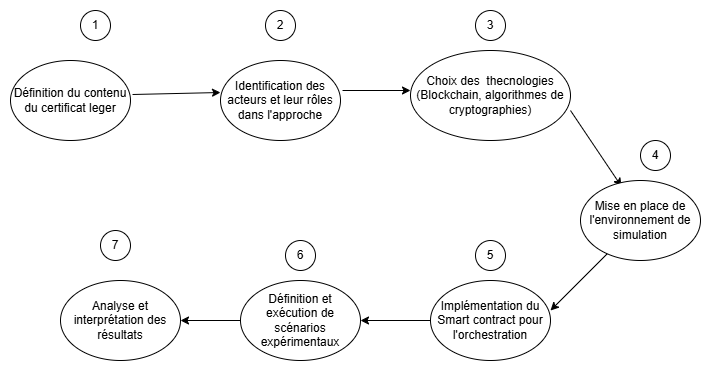
\includegraphics[width=\linewidth]{image/Demarche.png}
	\caption{Démarche Méthodologique}
	\label{demarche}
\end{figure}

\begin{enumerate}
    \item Définition du contenu du certificat léger, en tenant compte des contraintes des dispositifs IoT et des exigences de sécurité.
    \item Identification des entités impliquées et de leurs rôles dans le processus de gestion des certificats.
    \item Choix de la technologie blockchain et des outils techniques nécessaires à l’implémentation de l’approche proposée.
    \item Mise en place de l’environnement de simulation permettant de reproduire le comportement des différents composants du système.
    \item Implémentation du smart contract assurant l’orchestration du processus de validation et de gestion du cycle de vie des certificats.
    \item Définition et exécution de scénarios expérimentaux représentatifs des cas d’usage considérés.
    \item Analyse et interprétation des résultats obtenus à partir des métriques d’évaluation retenues.
\end{enumerate}

Cette démarche permet de relier de manière cohérente la conception de la solution à son implémentation et à son évaluation expérimentale. Nous donnerons plus de details ci-dessous. 

\subsection{Définition du contenu du certificat}

La première étape de la démarche consiste à définir le contenu du certificat utilisé dans l’approche proposée. Cette étape est fondamentale, car le certificat constitue l’élément central du mécanisme d’authentification et de confiance entre les entités du système.

L’objectif est de concevoir un certificat léger, contenant uniquement les informations strictement nécessaires à l’identification du dispositif et à la vérification de son authenticité, tout en garantissant un niveau de sécurité compatible avec les exigences des communications. Pour ce faire nous nous sommes inspire du certificats legers propose par \textbf{Garba et al.}\cite{garba2023lightcert4iots} qui contenait ces champs : 
\begin{itemize}
    \item UUID
    \item Clé publiaue 
    \item Date d'expiration
    \item Statut de validite
\end{itemize}
Au quel nous avons juste ajouter un champ supplementaire appele \textbf{Timestamp} pour recuperer le temps au quel a ete lance la requete d'enrolement pour prevenr les attaques de type rejeu.

\subsection{Identification des entités et de leurs rôles}

Une fois le contenu du certificat défini, la deuxième étape consiste à identifier les différentes entités impliquées dans le système et à préciser leurs rôles respectifs. Cette identification permet de structurer l’architecture globale et de clarifier les responsabilités de chaque composant. À ce niveau également, la structure des entités et des rôles proposée est fortement inspirée de celle de \textbf{Garba et al.} \cite{garba2023lightcert4iots}, mais elle s’en distingue par l’introduction d’une entité supplémentaire, à savoir le quorum de validation. Les entités considérées et leurs rôles sont décrits ci-dessous.

\begin{itemize}
    \item \textbf{Appareils IoT} : \\
    Les appareils IoT constituent les entités finales du système. Leur rôle principal est de générer localement le contenu du certificat léger auto-signé, incluant la clé publique et les informations d’identification minimales, puis d’envoyer une requête d’enrôlement à l’autorité locale d’enregistrement (LRA). Les appareils IoT sont également capables de prouver la possession de leur clé privée associée lors du processus d’enrôlement. Une fois enrôlés, ils peuvent établir des communications sécurisées avec d’autres appareils IoT. Concrètement, un appareil IoT peut être un capteur, une caméra intelligente, une imprimante connectée ou tout autre dispositif embarqué contraint.

    \item \textbf{LRA locale} : \\
    L’autorité locale d’enregistrement joue le rôle d’intermédiaire entre les appareils IoT et l’infrastructure blockchain. Elle constitue le point d’entrée du système pour les requêtes d’enrôlement des certificats. La LRA locale est responsable de la réception des requêtes émises par les appareils IoT, de la vérification des preuves de possession des clés cryptographiques et de la validation initiale du contenu des certificats légers. Après cette première vérification, la LRA transmet les informations nécessaires au mécanisme de validation distribuée, sans disposer à elle seule du pouvoir de décision final.

    \item \textbf{Quorum de validation} : \\
    Le quorum de validation est composé d’un ensemble de LRAs sélectionnées pour participer à un processus de validation distribuée. Chaque membre du quorum vérifie indépendamment les informations associées à une demande d’enrôlement et émet un vote ou une signature attestant de la validité du certificat proposé. L’objectif de ce quorum est de réduire la confiance accordée à une entité unique et de limiter l’impact d’une LRA compromise ou malveillante. La décision finale d’acceptation ou de rejet d’un certificat repose sur l’atteinte d’un seuil minimal de validations au sein du quorum.

    \item \textbf{Smart contract} : \\
    Le smart contract agit comme un orchestrateur du système de gestion des certificats. Il est déployé sur la blockchain et implémente la logique de sélection du quorum, de coordination du processus de validation et d’agrégation des signatures produites par les LRAs. Le smart contract est également responsable de l’enregistrement final des certificats validés ainsi que de la mise à jour de leur état en cas de renouvellement ou de révocation. Son exécution automatique garantit la transparence et l’auditabilité des opérations.

    \item \textbf{Blockchain} : \\
    La blockchain constitue le registre distribué et immuable du système. Elle assure le stockage de l’historique des certificats, incluant leur émission, leur mise à jour et leur révocation. Grâce à ses propriétés de décentralisation et d’immutabilité, la blockchain permet à toute entité autorisée de vérifier l’état d’un certificat sans dépendre d’une autorité centrale. Elle joue ainsi un rôle fondamental dans la gestion décentralisée de la confiance au sein de l’architecture proposée.
\end{itemize}


Les entités considérées incluent notamment les dispositifs IoT, les autorités locales d’enregistrement, le quorum de validation, le smart contract et la blockchain. La définition précise des rôles permet d’éviter les ambiguïtés fonctionnelles et de limiter les dépendances excessives entre les composants, contribuant ainsi à la robustesse et à la sécurité du système.Les autres  sections seront naturellement developper dans la suite de notre travail principalement dans l'implementation.


% \subsection{Approche adoptée}
% \begin{itemize}
%     \item Collecter des données I/Q en sortie de PA via simulation MATLAB/5G Toolbox.
%     \item Appliquer un prétraitement (normalisation, alignement temporel).
%     \item Concevoir une architecture NN optimisée pour la prédistorsion (taille, activation, régularisation).
%     \item Entraîner hors-ligne avec un ensemble d’apprentissage et de validation.
%     \item Évaluer la performance (ACLR, EVM, NMSE).
%     \item Comparer aux méthodes DPD classiques.
% \end{itemize}

\section{Approche proposée}

L’architecture globale de l’approche proposée est représentée par la Figure~\ref{architecture}. Cette architecture a été conçue afin de répondre aux contraintes spécifiques des environnements ......


%==================================================================================
\chapter{Implémentation, tests et résultats}
\section{Environnement logiciel et matériel}
\subsection{Environnement matériel utilisé}

L’implémentation et les expérimentations de l’approche proposée ont été réalisées sur une plateforme matérielle de développement standard, permettant de simuler l’ensemble des composants de l’architecture tout en garantissant des conditions de test reproductibles.

Les caracteristiques de la machine utilisée pour le développement et l’exécution des différents modules sont definis dans le tableau \ref{tab:env_materiel} ci-dessous.
\begin{table}[h]
\centering
\caption{Tableau machine et caractéristique}
\label{tab:env_materiel}
\begin{tabular}{|l|l|}
\hline
\textbf{Caractéristique} & \textbf{Valeur} \\ \hline
Mémoire vive (RAM) & 16 Go \\ \hline
Mémoire ROM (Stockage) & 1 To \\ \hline
Fréquence du processeur & 2{,}2 GHz \\ \hline
Système d’exploitation & Ubuntu 24.04 \\ \hline
\end{tabular}
\end{table}

\subsection{Environnement Logiciel Utilisé}

Cette section présente les principaux outils logiciels utilisés dans l’implémentation de l’approche proposée. Pour chaque logiciel, son rôle et son utilité dans le cadre de cette implémentation sont explicités.

\begin{table}[h]
\centering
\caption{Tableau environnement logiciel utilisé}
\label{tab:env_logiciel}
\begin{tabular}{|l|l|}
\hline
\textbf{Logiciel} & \textbf{Rôle / Description} \\ \hline
Contiki-NG & Environnement de simulation pour dispositifs IoT contraints \\ \hline
FastAPI & Framework web pour l’implémentation des services applicatifs et des LRAs \\ \hline
Ethereum & Blockchain public \\ \hline
Ganache & Blockchain locale de test pour le déploiement et l’exécution des smart contracts \\ \hline
Truffle & Framework de développement, compilation et déploiement des smart contracts \\ \hline
Docker & Conteneurisation des composants logiciels pour un déploiement reproductible \\ \hline
ProVerif & Outil de vérification formelle des protocoles de sécurité \\ \hline
\end{tabular}
\end{table}
\newpage

\subsection{Contiki-NG}

Contiki-NG est un système d’exploitation et un environnement de simulation dédié aux dispositifs IoT contraints. Il est utilisé dans ce travail pour simuler le comportement des dispositifs IoT participant au processus de gestion des certificats.


\begin{figure}[htb]
	\centering
	
\includegraphics[width=0.75\linewidth]{image/Contiki_logo_2RGB.png}
	\caption{Logo de Contiki-NG}
	\label{contiki}
\end{figure}

\subsection{FastAPI}

FastAPI est un framework web moderne et performant, utilisé pour l’implémentation des services applicatifs de l’architecture proposée, notamment les autorités locales d’enregistrement (LRAs).

Dans cette implémentation, FastAPI permet de définir des interfaces de communication légères et sécurisées entre les dispositifs IoT, les LRAs et les autres composants du système. Il offre un cadre structuré pour la gestion des requêtes d’enrôlement, la vérification des preuves de possession et la transmission des informations vers le mécanisme de quorum et le smart contract. Son efficacité et sa simplicité contribuent à réduire la latence des opérations critiques.
\begin{figure}[htb]
	\centering
	
\includegraphics[width=\linewidth]{image/logo-teal_FastAPI.png}
	\caption{Logo de FastAPI}
	\label{fastapi}
\end{figure}

\subsection{Ethereum}

Ethereum est une plateforme blockchain programmable permettant le déploiement et l’exécution de smart contracts. Dans ce travail, Ethereum constitue le modèle de blockchain de référence sur lequel repose l’architecture proposée pour la gestion décentralisée des certificats.

L’utilisation d’Ethereum se justifie par sa capacité à exécuter des contrats intelligents complexes, nécessaires à l’orchestration du processus d’enrôlement, à la coordination du quorum de LRAs et à l’enregistrement immuable des certificats. Le smart contract implémenté définit les règles de validation, d’agrégation des signatures et de gestion du cycle de vie des certificats, sans dépendre d’une autorité centrale.

Dans le cadre de l’implémentation, Ethereum n’est pas utilisé directement sur un réseau public, mais à travers un environnement local simulé. Ce choix permet de conserver le modèle de fonctionnement d’Ethereum tout en évitant les contraintes liées aux coûts de transaction, à la latence et à la variabilité des performances d’un réseau public. Ethereum constitue ainsi le socle conceptuel et technique de la solution proposée, tandis que Ganache est utilisé comme environnement d’expérimentation.

\begin{figure}[htb]
	\centering
	
\includegraphics[width=0.50\linewidth]{image/ethereum.png}
	\caption{Logo Ethereum}
	\label{ethereum}
\end{figure}

\subsection{Ganache}

Ganache est un environnement de blockchain locale utilisé pour le développement et les tests des smart contracts. Il permet de simuler le comportement d’une blockchain publique dans un cadre contrôlé et reproductible.

Dans ce travail, Ganache est utilisé pour déployer et tester le smart contract responsable de la gestion du cycle de vie des certificats. Il permet d’observer le comportement du système lors de l’enregistrement, de la mise à jour et de la révocation des certificats, sans les coûts et la latence associés à une blockchain publique réelle. Cet environnement facilite l’expérimentation et le débogage des interactions blockchain.
\begin{figure}[htb]
	\centering
	
\includegraphics[width=0.5\linewidth]{image/Ganache.jpg}
	\caption{Logo Ganache}
	\label{ganache}
\end{figure}
\newpage

\subsection{Truffle}

Truffle est un framework de développement pour les smart contracts. Il est utilisé pour la compilation, le déploiement et la gestion du cycle de développement des contrats intelligents implémentés dans ce travail.

Truffle fournit un ensemble d’outils permettant d’automatiser les phases de test et de déploiement du smart contract sur la blockchain simulée par Ganache. Il contribue à structurer le développement du composant blockchain et à assurer la cohérence entre le code du smart contract et les autres éléments de l’architecture.
\begin{figure}[htb]
	\centering
	
\includegraphics[width=0.5\linewidth]{image/truffle-seeklogo.png}
	\caption{Logo truffle}
	\label{truffle}
\end{figure}

\subsection{Docker}

Docker est une plateforme de conteneurisation utilisée pour isoler et déployer les différents composants logiciels de l’architecture proposée.

Dans cette implémentation, Docker permet de déployer de manière reproductible les services applicatifs, les autorités locales d’enregistrement et l’environnement blockchain. La conteneurisation facilite la gestion des dépendances logicielles, améliore la portabilité du système et garantit la cohérence des expérimentations réalisées lors de l’évaluation.
\begin{figure}[htb]
	\centering
	
\includegraphics[width=0.5\linewidth]{image/Docker (1).png}
	\caption{Logo Docker}
	\label{docker}
\end{figure}
\newpage

\subsection{ProVerif}

ProVerif est un outil de vérification formelle dédié à l’analyse des protocoles de sécurité. Il est utilisé dans ce travail pour vérifier formellement certaines propriétés de sécurité du protocole d’enrôlement et de communication proposé.

L’utilisation de ProVerif permet d’analyser des propriétés telles que l’authentification, la confidentialité des clés et la résistance aux attaques de type homme-du-milieu. Cette étape de vérification formelle renforce la crédibilité de l’approche proposée en apportant une validation théorique complémentaire aux évaluations expérimentales.

\begin{figure}[htb]
	\centering
	
\includegraphics[width=0.5\linewidth]{image/proverif.png}
	\caption{Logo Proverif}
	\label{proverif}
\end{figure}

\subsection{Justifications des choix des outils technologiques }

\section{Implémentation}
Détails étape par étape de la mise en œuvre.

\section{Simulation et tests}
\subsection{Simulation 1}
Conditions, paramètres, résultats.

\subsection{Simulation 2}
Conditions, paramètres, résultats.

\section{Analyse des résultats}
Courbes (ACLR, EVM), tableaux comparatifs, discussion.

%=======================
\chapter*{Conclusion et perspectives}
%\minitoc
\thispagestyle{fancy}


\addcontentsline{toc}{chapter}{Conclusion et perspectives}


\section*{Résumé}
Bilan des contributions.

\section*{Résultats majeurs}
Amélioration mesurée par rapport à l’état de l’art.

\section*{Perspectives}
Extension vers un apprentissage en ligne ou hybride.








%\renewcommand{\cftchapfont}{\bfseries}
%\renewcommand{\cftchappagefont}{\bfseries}
\renewcommand{\cftchappresnum}{\chaptername~} %affichera Chapitre dans la TOC
%\renewcommand{\cftchapaftersnum}{~}
\renewcommand{\cftchapnumwidth}{6em}


\cleardoublepage
%%=============================[Bibliographie]==============================================
\nocite{*} 

\printbibliography[heading=subbibliography, 
                    nottype=software,
                    nottype=softwareversion,
                    nottype=softwaremodule,
                    nottype=codefragment, 
                    title={\textsc{Bibliographie}
    }]
\thispagestyle{fancy} 

\newpage
%\dominitoc % Initialize the mini table of contents
\tableofcontents
\thispagestyle{fancy}

\end{document}


